% \documentclass{article}
\documentclass[twocolumn]{article}
\usepackage[utf8]{inputenc}
\usepackage{graphicx}
\usepackage{mathtools}
% \usepackage{multicol}
%\usepackage[letterpaper, margin=1in]{geometry}
\usepackage[letterpaper, top=2cm, margin=1in]{geometry}
\usepackage{listings}
\setlength{\columnsep}{0.5cm}


\title{6.858 Project: One Time Chat}
\author{Jake Barnwell, Andres Perez, Miles Steele}
\date{December 2015}

\begin{document}

\maketitle

%% things we should touch upon:

%% according to https://www.usenix.org/legacy/event/samples/submit/advice.html
%% original ideas: the new ideas our system introduces.

%% reality: have we implemented the system we proposed?

%% lessons: What have we learned? What? What do you mean?

%% choices: what were the alternatives considered at various points, and why were the choices made the way they were? 

%% context: what were the assumptions on which the work was made? Basically outline our threat model. 

%% focus: Does the introductory material contain excess baggage not needed for your main development?

%% The big ideas in our system is the fact that we are utilizing availability to the generation and storage of a lot of random bits 
%% We can copy stuff from our proposal
%%    https://docs.google.com/document/d/1_FF7lQLu9n2U8_IKfhBmUNniqJRTgcijVhL4yp7JJ1Q/edit
% \begin{multicols}{2}


\section{Abstract}
One Time Chat is a chat service that aims to be information-theoretically secure. Specifically, we propose a chat service that is built on top of a randomly-generated one-time pad. Furthermore, we explore limitations to this model, why one-time pad encryption isn't typically used in practice, and how we aim to resolve these issues.
%% http://ieeexplore.ieee.org/stamp/stamp.jsp?tp=&arnumber=6769090 %% 

\section{Introduction}
Users typically look to public-key cryptography for secure communication. While public-key cryptography is widely used and sufficiently secure in practice, it is not information-theoretically secure. The assumption behind the security of public-key cryptography is that factorizing integers is thought to be a computationally hard problem. However, this complexity has not been proven, and there are no gaurantees that this presumed one-way function will not be broken in the future.
 
Fortunately, encryption using a one-time pad has been proven to be completely information-theoretically secure (under the right circumstances). We propose a chat service that is built upon a large\footnote{
In practice, one that will last a lifetime.
}
one-time pad, allowing two (or more) users to securely communicate with each other with guaranteed confidentiality and integrity.

\subsection{Usage of a One-time Pad}
Suppose Alice wants to send Bob a message. In order to guarantee to both Alice and Bob that her message $m_1$ will be securely\footnote{
that is, in a manner in which no other user will be able to infer the content of the message
}
transmitted to Bob using a one-time pad, they must first agree on a secret pad $p_{1}$. After Alice prepares the message, she \emph{encrypts} her message by computing the \emph{ciphertext} $c_{1} = m_{1} \oplus p_{1}$, where $\oplus$ is the bit-wise XOR operator. Bob, when receives the ciphertext $c_1$, can compute the original message $m_1 = c_1 \oplus p_1$.

This pad $p_1$ \emph{cannot} be reused, and must be immediately destroyed. Reusing any bits from $p_1$ breaks the one-time assumption about the pad, and renders prolonged communication cryptographically insecure.

\subsection{Drawbacks of the One-time Pad}
Though the one-time pads offers, in theory, completely secure communication, care must be taken to implement and use the system correctly. There are three primary issues with one-time pads that must be addressed appropriately to ensure security:
\begin{enumerate}
\item The pad must be made up of \emph{random} bits of data. If the pad's bits are not truly random, then an adversary could obtain information about the message by observing the ciphertext. Pseudo-random number generators (PRNGs) are not sufficient for creation of one-time pads, since PRNGs rely heavily or entirely on deterministic functions; even very chaotic functions, like Mersenne twisters, are easily dismantled if an adversary can pinpoint a seed.
\item The users may \emph{never} reuse the pad (or the relevant portion of the pad). Suppose two messages $m_{1}$ and $m_{2}$ are encrypted using the same pad $p$, resulting in $c_1$ and $c_2$, respectively. Then, we find that
\[
c_{1} \oplus c_{2} = p \oplus m_{1} \oplus p \oplus m_{2}
= m_1 \oplus m_2
\]
Since an adversary knows both $c_1$ and $c_2$, she clearly knows $m_1 \oplus m_2$, which means that she has information about both messages. This is not secure.
\item Each time a message is encrypted with a pad, the pad must be the same length as the message. In other words, before two users can communicate with each other, they must have already established a shared pad that is of sufficient length to encrypt all of their intended messages.
\end{enumerate}
Together, these three issues make one-time pads less preferred for encryption than other more popular schemes, even though one-time pads are information-theoretically secure.
%issue one: random pad
%issue two: no reuse pad
%isue three: length of pad = length of mesage.

\section{Design}
We believe that much of the inconvenience of using one-time pads can be solved by generating and sharing a pad that is long enough to encrypt all messages that a user could feasibly send in his lifetime. We hypothesize that a pad on the order of 1 terabyte (TB) in size would be enough to encrypt every text message for the rest of his life. \footnote{
See Section~\ref{sec:encryption} for details.
}

Our design involves two users\footnote{
``Group chat'' (i.e. chat among three or more users) is implemented as a simple extension on top of two-way secure chat. See Section~\ref{sec:clientexample}.
}
meeting in person and generating a pad from a local source of randomness, e.g. UNIX's \texttt{/dev/random}. We have noticed in practice that this can take a while, but the wait is well worth it, and users could certainly find ways of occupying themselves while the pad is generated. Users then (presumably securely) transfer the generated pad to their local storage device, and part ways.

At this point, the users can store their shared one-time pad on hardware devices and communicate using our chat system. Since both users share the same stream of random bits, they can achieve perfect security under certain threat model assumptions, as long as they synchronize their use of the pad.

\subsection{Definitions}
We define the following terms:
\begin{itemize} \itemsep0em 
  \item \textbf{User} Person using the chat service.
  \item \textbf{Client} Command line interface and chat software, typically run on a computer.
  \item \textbf{Device} Separate entity that stores the pad and other data; in our case, a Raspberry Pi or, for proof of concept, emulated on the computer.
  \item \textbf{Server} Message-Relay Server that ferries messages between clients.
  \item \textbf{Pad} Very large one-time pad: shared random bits between two users, and associated metadata. Stored on the device.
  \item \textbf{Pad segment} Some small portion of the pad, used to help encrypt a message.
  \item \textbf{Secrecy} Inability for an attacker to guess any bits of a message.
  \item \textbf{Integrity} Inability for an attacker for forge or modify a message, or to spoof a phony sender for a received message.
  \item \textbf{Security} Catch-all phrase used to declare both secrecy and integrity.
  \item \textbf{RNG} Random number generator. A service that (somehow) generates random numbers.
  \item \textbf{HRNG} Hardware random number generator. An RNG service that uses hardware input to help generate ``truly'' random data.
\end{itemize}


\subsection{Goals}
One Time Chat has been designed to address several specific goals that we have decided are important. We enumerate our goals below:
\begin{itemize}
\item \textbf{Confidentiality}: Messages sent from user A to user B should only be viewable by users A and B.\footnote{
Or, in the case of a group message, by exactly the users in the group.
}
More strongly, an attacker should not be able to infer any amount of information about the message, except for possibly its length.
\item \textbf{Integrity}: The receiver of a message should be able to know, with an extremely high probability, if an attacker (e.g. a man in the middle) modifies the message that is received. Furthermore, the receiver must be able to know, with an extremely high probability, that the message originated from who she thinks it did.
\item \textbf{Security Against Malicious Server}: A malicious chat server should not be able to drop, modify, or replay packets without the receiver knowing.
\item \textbf{Security Against Malicious Client}: If the user is running the chat client on a malicious computer, it \emph{is} possible that the the malicious computer can eavesdrop (e.g. with a keylogger) on the plaintext message typed by the user ryin, modify the message and/or recipient[s], or drop the message entirely before it is even encrypted or sent over the network. Besides these infractions, the client \emph{must not} be able to modify the encrypted message (once it is encrypted), or be able to read any part of the user's pad whatsoever. Furthermore, any infraction made by the malicious client at this point must not negatively impact the security of future messages sent by the user via non-compromised clients.\\
Similarly, the malicious client may read the decrypted message from a received packet, or modify the sender tag, since the message will likely be shown on the screen of the client to the user. Besides this, the client should not be able to read or know any bits of either user's pad, nor negatively impact the security of future messages received by the user via non-compromised clients.
\end{itemize}

\subsection{Non-Goals}

\begin{itemize}
\item \textbf{Availability}: We do not provide any guarantees or solutions for availability of One Time Chat. Though it is very important for a chat service to have a high up-time, we did not consider it necessary to show this proof of concept in our chat system. We are certain that if an adversary, or group of adversaries, tried hard enough, they could DOS our server and deny access to users.
\item \textbf{Server Security}: The security of the server is not that relevant to this project. There are most likely several bugs and vulnerabilities in the server code, leaving it open to attacks of various kinds. This is not an issue, and indeed aligns with our assumptions that a server may be malicious, malformed, or just not very reliable.
\end{itemize}

\section{Threat Model}
We assume that the server has bugs and vulnerabilities, is susceptible to attacks, and is generally untrusted. The server may drop or modify packets of its choosing. While we do \emph{allow} for the possibility of the server dropping or modifying every single packet, we typically assume that it relays a reasonable amount of messages untarnished.\footnote{
For example, if Bob never receives a message from Alice, it is difficult for Bob to know if the server is dropping all of Alice's packets or if she just never sent him anything.
}
We can even assume that the server logs every packet that is sent through it; can store them indefinitely; can distribute them to other users, adversaries, servers, or clients; and replay these packets at a later point to try to get them decrypted, somehow.

We allow for the possibility that certain clients the user uses are untrusted, but not all of them. We recognize that a malicious client can still read a user's incoming or outgoing plaintext messages, since the user types on the client computer and reads messages on the screen. However, when a user is on a malicious client, future and past messages are not vulnerable,\footnote{
For example, if a malicious server logged several previous (encrypted) messages while both users were using non-malicious clients, and Alice was now using a malicious client, the server might send those encrypted packets to the malicious client to try to get them decrypted. Even if the server never sent those stored packets to the recipient, One Time Chat has systems in place to protect against this attack.
}
only current ones transmitted via the current client.

We assume that the device itself is fully trusted, and is not malicious. Furthermore, the connection between the device and the client is trusted.

The pad, located on the device, is assumed to be randomly generated using an RNG service. We assume the pad is kept secure (only the two relevant users have access to it), and that no one else knows anything of the bits of the pad, except for possibly its length. 

If the device is physically compromised (e.g. stolen by an adversary) or the secrecy of the pad is broken, we do not guarantee the security of any messages, past, present, or future. This should be obvious: after all, the pad is the secret key between the users.

The RNG service that creates the pad is trusted, and is truly random.\footnote{
Even with the HRNG there may still be biases, but treat it to be unpredictable in our analysis.
}
It is not pseudo-random. Lastly, we assume there is a way to securely transmit the pad data to the device, if the pad was not generated on the device.

We assume that the correct use of One-time Pads is information-theoretically secure in its secrecy but provides no integrity guarantees of its own.

The SHA256-based HMAC is assumed to be a computationally hard to reverse. If this assumption is broken, our system still preserves secrecy. We are not sure whether our system still guarantees the integrity of messages if HMAC is broken. See Section~\ref{sec:encryption} for details.

Besides the one-time pad and SHA256-based HMAC, we do not rely on other encryption schemes. As such, we are allowed to assume that such encryption schemes are broken.


\section{Encryption}
\label{sec:encryption}

In order to securely send a message from Alice to Bob, Alice's device encrypts and signs the message, resulting in what we call a package. A package is defined according to the following scheme:
\begin{align*}
package &\coloneqq index || (p_{body} \oplus body) \\
body &\coloneqq ciphertext || tag \\
ciphertext &\coloneqq p_{text} \oplus message \\
tag &\coloneqq HMAC(p_{key},ciphertext) \\
\end{align*}
Lengths of the components:
\begin{align*}
|message| &= |ciphertext|+|p_{text}|\\
|body| &= |p_{body}| \\
|tag| &= 32\, bytes \\
|p_{key}| &= 16\, bytes \\
\end{align*}

A package is composed of an index, and a body. The index allows the user receiving the package to infer from where in the pad to construct pad segments $p_{text}, p_{body}, p_{key}$. The body is our way of encrypting a message and providing integrity to the packet. The rest of this section aims to explain why we think this scheme accomplishes our goals.  

Our system requires $2\cdot |message| + 48$ bytes of pad to encrypt and securely send a message (see Section~\ref{sec:encryption}). With the (very generous) assumption that an average text message is 100 bytes (i.e. 100 characters long), if a user had a 1 TB pad, he could could send over $150000$ such texts \emph{per day} for the next 80 years.\footnote{
Alternatively, he could choose to send up to 4 or 5 Vlad the Impaler articles per day.
}

With modern technology, this is not an unreasonable amount of storage. A cursory search online reveals that a 512 GB USB drive can be found for roughly \$20. Anyone who is genuinely concerned about security would likely be willing to spend that much or more for a lifetime guarantee of secure communication.

\subsection{Confidentiality}
It is impossible to deduce $message$ given $message \oplus p_{text}$
as long an adversary has not obtained $p_{text}$, and it is impossible to deduce $body$ from $body \oplus p_{text}$. Since our threat model assumes an adversary does not have access to the pad, it is impossible for an adversary to know what $message$ and $body$ are. We do not care to provide confidentiality of $index$, because without the pad this piece of information does not reveal critical information. 

\subsection{Integrity}
We argue that $body$ provides integrity of the package. An adversary knows where in $package$ $ciphertext$ lies (though they don't know what $ciphertext$ is since it is encrypted with part of $p_{body}$). Since one-time encryption is malleable, adversaries know that flipping bits in $ciphertext$ will flip bits in $message$. However, if an adversary doesn't change $tag$, then with high probability the user would be able to tell that $ciphertext$ has been changed, because the modified $ciphertext$ would fail to have the same HMAC. For the adversary to fool the receiver, they would thave to change the tag as well. Because the HMAC has a private key that the adversary does not know $p_{key}$.
If an adversary changed the bits corresponding to $ciphertext$, the tag would reflect that change. In other words, when users take they keyed HMAC of the modified $ciphertext$, with high probability it won't equal the  

We guarantee good integrity.
% < say more.

\subsection{Description}
% < Packaging description.
% < pseudo code of packaging

\subsection{Attacks}
Here we walk through some potential attacks and show how secure our scheme is against them.

\subsubsection{Snoop Original Message}
If an attacker can intercept all network traffic between two clients, they should not be able to recover the original message.
We can support this guarantee even under the assumption that the Sha256-based HMAC we use for integrity is completely broken.
Assume for the analysis of this attack that we use the identity function as the HMAC, as the most pessimistic scenario.
% < perfect secrecy

\subsubsection{Malleability Attack}
If an attacker can intercept and modify all network traffic between two clients, they should not be able to flip any bits in the underlying message and still pass the integrity check step.
For this attack we assume a worst case in which the attacker knows the full plain text of the message and the message is only 1 bit long.
We assume, however, that the HMAC we use is hard to fake without a known key.
% < ... should be ok
Our protection against malleability is less strong than our secrecy guarantee because it depends on the properties of HMAC.

\subsubsection{Extension Attack}
If an attacker can intercept and modify all network traffic between two clients, they should not be able to add additional bits to the underlying message and still pass the integrity check step.
% < alignment also helps us here, but it needn't be the main reason we're safe
% < integrity check should fail

\subsubsection{Pad Re-use}
In any one-time-pad based scheme, it is vitally important that each bit in the pad is only used to encrypt once, ever.
Our system defends against pad re-use by having the device manage which bits have been used to encrypt and decrypt during the lifetime of the pad.
Because the pad is stored on two devices, it is critical to make sure that even if the devices cannot communicate, they do not encrypt messages with the same bits as each other. This is why we divide the initial pad in half and dedicate each half for sending from one device.

% < software doesn't send from same pad bits ever
% < we only release information from decrypted if integrity check succeeds
% < describe actual possible attack given integrity spoofing!

\section{Implementation}
One Time Chat is implemented using three separately-running python programs.
The client software runs on a laptop or desktop which the user places a reasonable amount of trust in. It hosts the chat UI and communicates with the user, pad device, and server.
The pad device holds the one time pad data for the user and their contacts, as well as relevant metadata. It communicates through a private, secure channel with the client.
The message relay server is an untrusted server used to transfer messages between clients. See Figure \ref{fig:systemd}.

\begin{figure}[htp]
\centering
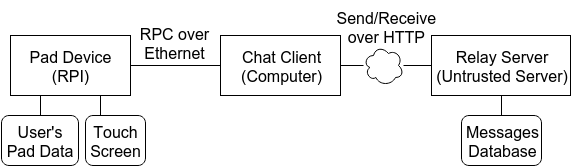
\includegraphics[width=2.8in]{system-diagram}
\caption{System Diagram}
\label{fig:systemd}
\end{figure}

\subsection{Pad Structure and Storage}
The pad data for a pair of users is stored in two files in the device's file system. Suppose two users, Alice and Bob, have set up a shared pad (see Section~\ref{sec:padgen} for details on pad generation) to communicate with each other. Alice's device stores two files: \texttt{alice.bob.random.store} and \texttt{alice.bob.random.metadata}; Bob has oppositely named files.

The store file (\texttt{alice.bob.random.store}) stores the randomly-generated pad bits. Alice and Bob's store files are identical, i.e.
\texttt{alice.bob.random.store == bob.alice.random.store}. Whenever pad segments are requested to help encrypt/decrypt a message, handler code stored on the device interfaces with the store files to retrieve the appropriate pad bits.

The metadata file \texttt{alice.bob.random.metadata} stores certain information about the pad, the contact, and how many bits of the pad have been used for encryption and decryption:

\begin{itemize} \itemsep0em 
  \item[] \textbf{uid} User ID of user
  \item[] \textbf{rid} User ID of contact
  \item[] \textbf{store\_filename} Filename of the random store
  \item[] \textbf{metadata\_filename} Filename of this metadata file
  \item[] \textbf{n\_bytes} Total number of shared pad bytes
  \item[] \textbf{rservice} Service used to generate the bytes (\texttt{random} or \texttt{urandom}). In practice this should always be \texttt{random}.
  \item[] \textbf{split\_index} Index dividing the two halves of the pad
  \item[] \textbf{direction} Direction of encryption (1 means encrypt starting at index 0 and moving forward, means encrypt starting at index \texttt{n\_bytes - 1} and moving backwards).
  \item[] \textbf{encrypt\_index} Index of pad to start encrypting from the next time a pad segment is requested
  \item[] \textbf{decrypt\_log} A log of all decryption requests the device has seen; each decryption request is of the form \texttt{i-j} which signifies that pad segment from $i$ to $j$ was requested to decrypt.
  \item[] \textbf{decrypt\_max} Maximum index for a pad segment that has been requested for a decryption. Note that if direction is 1, you \emph{decrypt} backwards (since your contact has direction -1), this is actually a minimum.
  \item[] \textbf{n\_eles} Number of fields in this metadata, including this one.
  \item[] \textbf{checksum} Hash to help ensure the metadata wasn't accidentally modified. Not intended to protect against a malicious adversary.
\end{itemize}

The reason we split the pad into two is so that messages can be sent from Alice to Bob and from Bob to Alice asynchronously: if Alice sent $m_A$ with index $i_A$ to Bob, while at the same time Bob sent message $m_B$ to Alice with index $i_B$, then if both users were reading from the same portion of the pad, there could be interference: both could, for example, try to use the same portion of the pad to encrypt, which breaks the security of a one-time pad. By splitting up the pad, each user has a dedicated set of bits to send (encrypt) from, and the recipient knows where in the pad to decrypt from when they see an incoming message from the sender.

Alice encrypts from index 0 moving forward in the top half of the pad (delimiter stored by the \texttt{split\_index} field), and Bob encrypts from index \texttt{n\_bytes - 1} moving backward in the bottom half the pad. Similarly, when Alice decrypts a message (from Bob), she reads Bob's half of the pad, in reverse; and when Bob decrypts a message, he reads Alice's half of the pad in the forward direction. See Figure \ref{fig:padsplit} for a helpful diagram.

\begin{figure}[htp]
\centering
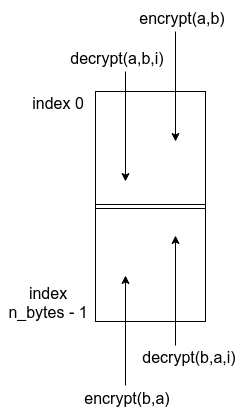
\includegraphics[width=1.5in]{padsplit}
\caption{Pad Layout. \texttt{encrypt(a,b)} means that \texttt{a} is sending to \texttt{b} and needs to encrypt. Similarly, 

\label{fig:padsplit}
\end{figure}

The reason we have the encryption directions moving in opposite directions towards the center of the pad is so that the \texttt{split\_index} can be appropriately modified if, for example, Bob has run out of encryption pad but Alice still has half of hers. However, this feature has not been implemented in the current version.

Obviously, Bob's and Alice's metadata files differ. Each keeps track of messages it has been asked to decrypt, as well as what is the next index of the pad it should use to encrypt.

For example, if Alice has just received a new pad and has requested a pad segment of length 10, the device checks the direction and encrypt index of her metadata (sees that they are 1 and 0, respectively), and returns \texttt{pad[0:10]}, and then updates the encrypt index to 10 so it knows where to start the next time.

When Bob receives the encrypted message (also included is the requested \texttt{index}, i.e. a decryption index), he checks his metadata file to see what direction and which half the pad to look at, and then requests the pad segment \texttt{pad[decrypt\_index:decrypt\_index+len(msg)]}. The range of indices is stored into the \texttt{decrypt\_log}, and \texttt{decrypt\_max} is updated.

The decryption log and max indexes are stored to help detect dropped packets and replay attacks.

\subsection{Pad Generation}
\label{sec:padgen}
We use the \texttt{/dev/random} service to generate the random bits of our pads. Because \texttt{random} tries to generate bits based on stored entropy, it often blocks while waiting for more entropy, making it very slow to generate more than a few hundred bytes of data. To remedy this situation, we have purchased a hardware RNG (HRNG) device, a USB stick that helps seed \texttt{random} by generating randomness based on the emissions between two physical diodes. Even then, number generation is very slow for more than several megabytes. However, other more expensive HRNG devices would be much faster.

Note that for development and debugging, we often used \texttt{urandom} since it is much faster.

Figure \ref{fig:genpad} shows an example of generating an (insecure) pad from urandom.

\begin{figure}[htp]
\centering
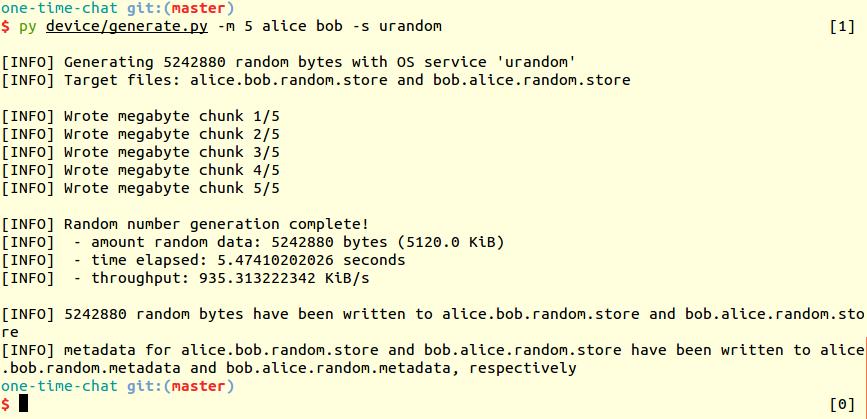
\includegraphics[width=3in]{generate}
\caption{Generating A Pad}
\label{fig:genpad}
\end{figure}


\subsection{Device (Pad Device)}
The pad device is a device dedicated to storing and mediating access to the one time pad data for a user and their contacts. Each user has one device which they are responsible for keeping safe. A user initializes their device with a shared pad for each contact they wish to communicate with.

Ideally, a Raspberry Pi would be used to run the device code and connect to the client computer through an ethernet cable. We got that to work for a little while. But we have had so much trouble with that we chose to run device software on the same computer as the client software. This eliminates the security benefits of having a dedicated device, but the code is still implemented in such a way that it is easy to run it on a separate device. For the analysis, we assume that this part is working.


\subsubsection{Packaging and Unpackaging}
The pad device is responsible for encrypting and decrypting messages. The encryption and decryption methods are in \texttt{device/crypto.py} with some tests in \texttt{device/test\_crypto.py}. See Section~\ref{sec:encryption} for the details of the encryption scheme. The crypto implementation relies on a simple xor function and on Python's built-in Sha256-based HMAC from the \texttt{hmac} module.

The two crypto functions used by the device are package and unpackage which when given message
data and pad data secure and unlock messages. These are base64 encoded for transport convenience when
returned to the client.

\begin{lstlisting}
package(index, message,
  p_text, p_body, p_tag_key):
unpackage(package,
  p_text, p_body, p_tag_key):
\end{lstlisting}

\subsubsection{Confirmation}
A malicious client might get a connection to the pad device. In this case, to defend the pad against malicious client software, a touchscreen on the raspberry pi is used to ask the user whether it is ok to use pad bits to encrypt and decrypt messages. This is a trade-off as it is an inconvenience to the user, but makes client-based attacks based on brute force almost impossible.

\begin{figure}[htp]
\centering
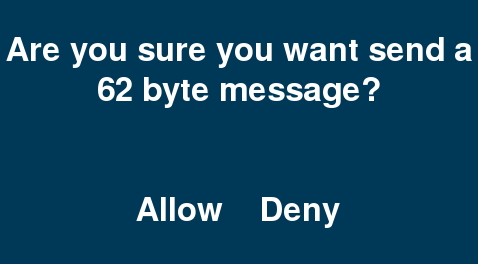
\includegraphics[width=2in]{confirm}
\caption{Confirmation dialog on device screen.}
\end{figure}

\subsubsection{RPC Interface}
The client communicates with the pad device via an HTTP server running on the device. The server is not accessible to the internet, but is available through the ethernet cable. Or as a local service when running on the same machine as the client.

The RPC server is an HTTP server which has a client that can be used as if it were a normal python module
from the client. Arguments and return values are sent as JSON.
This RPC server currently allows two methods, \texttt{package} and \texttt{unpackage}.
Those methods are responsible for asking the user for confirmation, getting pad data from pad storage, feeding it to the crypto functions, and returning the result. Any unexpected errors that occur are hidden from the client so that in the case of a programming error on the device, no sensitive information is leaked through errors.

\begin{lstlisting}
package(src_uid, dst_uid, plaintex):
unpackage(src_uid, dst_uid, package):
\end{lstlisting}

\subsubsection{Logging}
The device logs suspicious occurrences in a device-local log file.
All log entries have a timestamp and description of the error as well as
additional information about the messages involved.

Anytime the message integrity check fails (mismatched HMAC), the event
is logged.

If a message is received which uses a pad index that was used before,
this event is logged on the device (in addition to instructing the client
to display a warning).

If a pad index appears to have been skipped the event is logged
(in addition to instructing the client
to display a warning).

\begin{figure}[htp]
\centering
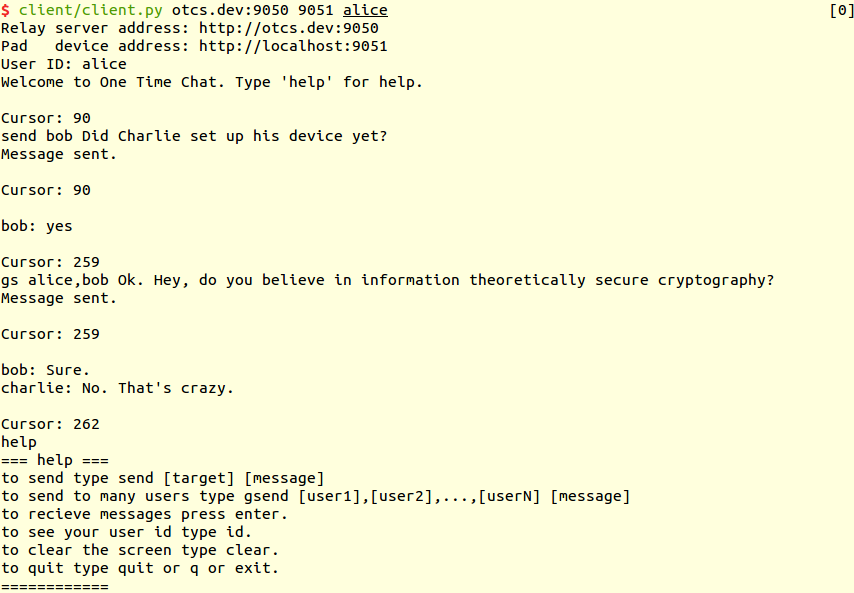
\includegraphics[width=3in]{sample}
\caption{Example Client Use}
\end{figure}
\label{sec:clientexample}

This log exists on the device and is inaccessible from outside.
The hope is that this log could provide some help in forensics
and damage analysis in the event of a known compromise.


\subsection{Chat Client}
The chat client presents a command line interface to the user for sending and receiving messages. It communicates with the device to request encryption and decryption, and exchanges encrypted messages with a relay server.

To start the client a user gives it as parameters the URL of the chat server, the URL of the device RPC channel, and their username.

\begin{figure}[htp]
\centering
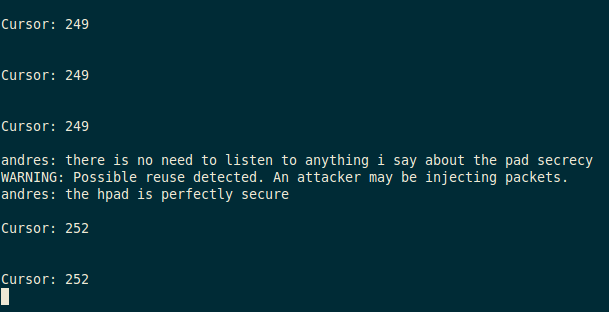
\includegraphics[width=3in]{reuse}
\caption{Detecting Reused Pad Data}
\end{figure}

The messaging-related client commands are listed below.\\
Send a message:\\
\-\ \-\ \textbf{send} [target] [message]\\
Send to multiple:\\
\-\ \-\ \textbf{ms} user1,user2,... [message] (multisend)\\
Define a group:\\
\-\ \-\ \textbf{group} [groupname] user1,user2,...\\
Send to group:\\
\-\ \-\ \textbf{gs} [groupname] message\\
Receive messages:
Press enter.


\subsection{Message Relay Server}
The relay server is an untrusted server which relays messages between chat clients.
It is implemented as a simple HTTP server with a single table for messages.

The server is not designed to be secure at all, but to be the minimum to demonstrate that
the rest of the system could work. It serves over HTTP with no authentication at all.
This is consistent with our threat model of not trusting the server but if One Time Chat were to be effectively used then a server with additional security measures would be required. The implementation is in \texttt{server/server.py} and stores messages for delivery in \texttt{server/database.db}.

The server provides the following endpoints for clients:
\begin{lstlisting}
/check: Make sure server is up.
/send: Send a message between users.
  - sender_uid
  - recipient_uid
  - contents
/getmessages: Get messages for a user.
  - recipient_uid
  - start_ref
\end{lstlisting}

Each message is assigned a ref number which clients keep track of in order
to fetch only messages they have not seen before from the server.
The latest ref is fetched from the server each time the client starts.



\section{Conclusion}
At the end of the day, we have implemented our own chat service, and our own cryptography. In other words, we have broken the first rule of cryptography which is don't write your own cryptography. As we iterated through the design of our protocol we learned how subtle details in protocol could lead compromises in confidentiality and integrity. As it stands we believe our system is secure under our threat model, and that our approach in sharing a large pad on a secure device is close step to information theoretically secure communication.


% \end{multicols}
\end{document}
